\subsubsection{Diseño de la interfaz}

La interfaz corresponde a la fase de diseño con el usuario del enfoque RAD. Se diseñó en dos pasos: la paleta de colores y los mockups de baja fidelidad en Excalidraw; el prototipo visual se construye en el desarrollo. Las pantallas cubren las acciones principales de cada rol identificadas en el Objetivo 1: para la secretaria, la agenda y la atención en recepción; para el odontólogo, sus citas y el registro de la atención.

\paragraph{Paleta de colores}

La paleta se deriva del logo del Centro Odontológico Bellidental, de un único azul (\texttt{\#143F76}). A partir de él se construyó una escala de azules, desde el tono más profundo para la barra lateral y los títulos hasta el casi blanco de los fondos. Como contraparte se eligieron tonos cálidos fuertes y antagonistas (ámbar, terracota, verde azulado e índigo), reservados para las acciones principales y los estados de la cita (Figura~\ref{fig:ob2_paleta}).

\begin{figure}[H]
\centering
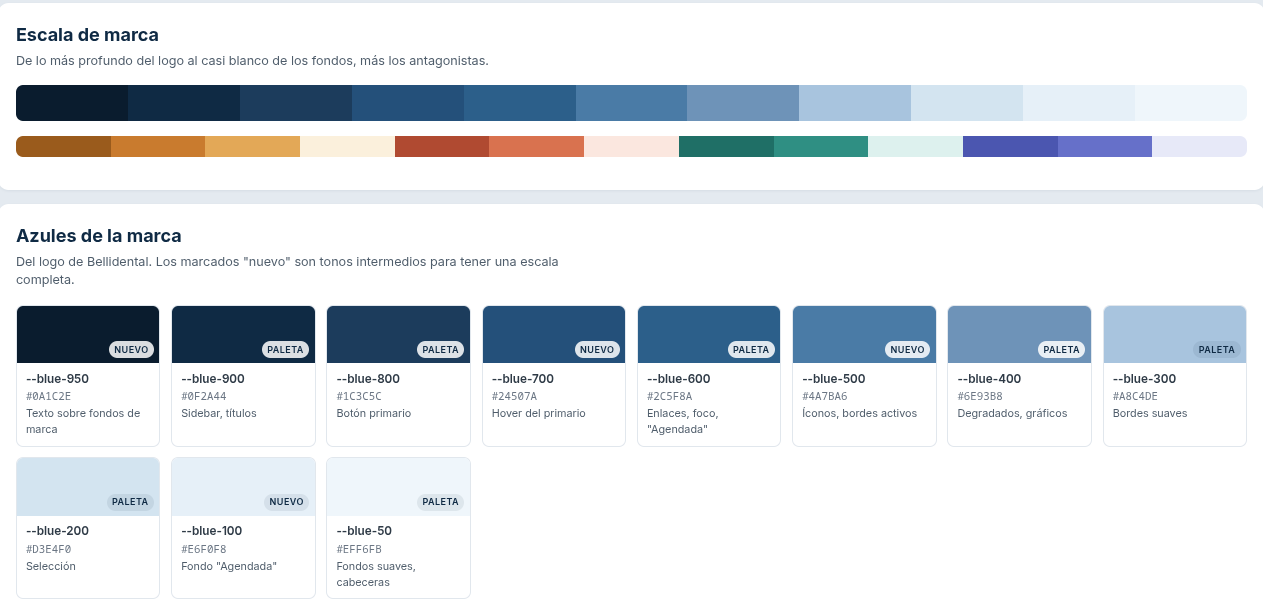
\includegraphics[width=\linewidth]{img/Paleta_Colores.png}
\caption{Paleta de colores}
\label{fig:ob2_paleta}
\end{figure}

\paragraph{Mockups}

Los mockups fijan la distribución de cada pantalla: la barra lateral por rol, el buscador de pacientes y la próxima cita en la cabecera. En la agenda de la secretaria (Figura~\ref{fig:ob2_mockup_agenda}), cada cita se marca con el color del profesional (RF07); en la atención del odontólogo (Figura~\ref{fig:ob2_mockup_atencion}), los datos del paciente, los antecedentes y el odontograma ocupan una sola pantalla, en reemplazo de la ficha rápida y su transcripción (PC1 a PC3).

\begin{figure}[H]
\centering
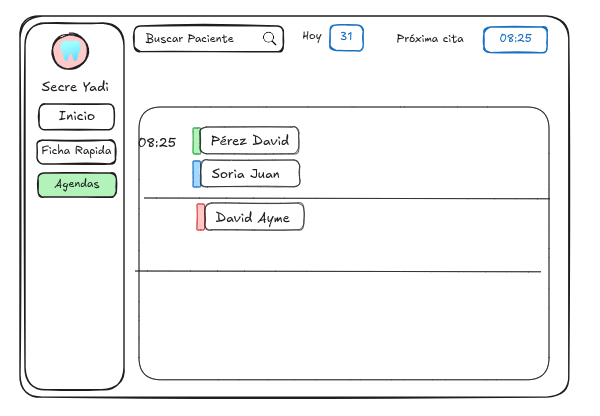
\includegraphics[width=0.7\linewidth]{img/Mockup_Agenda_Secretaria.png}
\caption{Mockup de la agenda de la secretaria}
\label{fig:ob2_mockup_agenda}
\end{figure}

\begin{figure}[H]
\centering
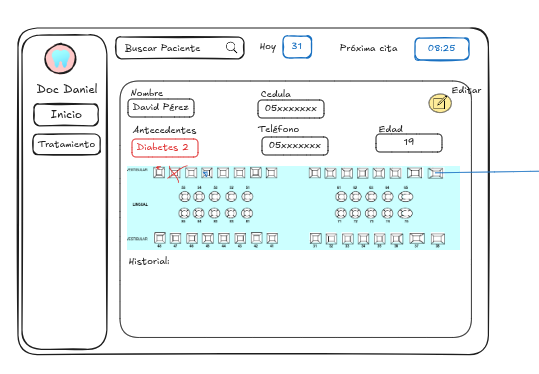
\includegraphics[width=0.7\linewidth]{img/Mockup_Atencion_Odontologo.png}
\caption{Mockup de la atención del odontólogo}
\label{fig:ob2_mockup_atencion}
\end{figure}
